\documentclass[10pt]{article}

\usepackage[margin=1.5in]{geometry}
\usepackage{graphicx}
\usepackage{natbib}
%correct punctuation for MBE
\bibpunct[,]{(}{)}{;}{a}{}{,}

\usepackage{amsmath}

\renewcommand{\bottomfraction}{.9}
\renewcommand{\topfraction}{.9}
\renewcommand{\textfraction}{0.1}
\renewcommand{\floatpagefraction}{.9}

\linespread{1.1}
\begin{document}

\title{\textbf{(working title) Filtering with Guidance is pretty useless}}
\author{Stephanie J. Spielman$^{1*}$ and Eric T. Dawson$^{1}$ Claus O. Wilke$^{1}$}
\date{}

\maketitle
\noindent
Address:\\
$^1$Section of Integrative Biology and Center for Computational Biology and Bioinformatics. The University
of Texas at Austin, Austin, TX 78731, USA.\\

\bigskip
\noindent
$^*$Corresponding author\\
$\phantom{^*}$Email: stephanie.spielman@utexas.edu\\

\bigskip
\noindent
Manuscript type: research article

\bigskip
\noindent Keywords: multiple sequence alignment, alignment filters, sequence simulation, positive selection inference

\newpage
\begin{abstract}
	People are really into masking alignments these days. Active development of methods. Here, we comprehensively test one common masking method and show that it's probably not as awesome as you thought. Is it bad? Probably not. But is it going to make or break you? Also no. Is it worth your time? Doubtful. Plus the actual guidance is pretty damn buggy, and that's ridiculous.
\end{abstract}


\section*{Introduction}
Constructing a multiple sequence alignment (MSA) represents the first step of analysis in most studies of molecular evolution, namely phylogenetic reconstruction and evolutionary rate inference. Recently, several studies have shown that poor MSA quality can significantly hinder accuracy in such downstream analyses \citep{Jordan2011, MarkovaRaina2011, Dwivedi2009, Talavera2007, Ogden2006}. In particular, the elevated false positive rates incurred during positive selection inference when using an alignment of poor quality has been a troubling observation  \citep{Jordan2011, Privman2012, Schneider2009, Fletcher2010}. As a consequence, many have advocated applying an alignment filter to MSAs before their use in such analyses. Such filters, which include GBLOCKS \citep{Castresana2000} and T-Coffee \citep{Notredame2000}, locate   putatively poorly aligned regions in alignments, thereby allowing users to curate their alignments to maximize signal. The hope is that culling unreliable positions and/or columns from MSAs will yield increased accuracy in positive selection inference, without excessively sacrificing power.

One widely used \textbf{(should i cite some papers that use guidance?)} software for alignment filtering is Guidance \citep{Penn2010}. Guidance bootstraps alignments by sampling variants in the alignment guide trees. Ultimately, Guidance derives a confidence score for each position in the alignment (see Penn et al. for details). Users can then ``mask" (i.e. replace with an ambiguous character such as ``?") positions with scores below a certain threshold, thereby removing residues that cannot be confidently placed in the alignment. This method is fairly conservative, as particular positions of low confidence can be removed rather than entire columns. Moreover, recent simulation studies have demonstrated that filtering poorly aligned residues with Guidance may confer increased accuracy when inferring positive selection \citep{Jordan2011,Privman2012}. 

Even so, while Privman et al. \citep{Privman2012} found dramatic improvements in positive selection inference when applying the Guidance filter, Jordan and Goldman's \citep{Jordan2011} comprehensive study on alignment methods and filtering found that Guidance yields modest, if any, effects on this inference. In particular, they reported that, at typical protein divergence levels or insertion/deletion (indel) rates, Guidance offers few benefits to positive selection inference; while the Guidance filter did not obscure signal, neither did it improve inferences. Alternatively, at extremely high divergence levels (1.8 mean path length) or indel rates (0.2 indel/substitution events), Jordan and Goldman found that Guidance significantly boosted true positive rates. While these results are compelling, protein sequences used in positive selection studies, however, rarely, if ever, contain sequences separated by such high divergences; the MPL for an average mammalian gene tree is only about 0.05 \textbf{citation needed maybe?}, or $1/36th$ the divergence level at which Jordan and Goldman detected improvements when using the Guidance filter.

Motivated by these apparent discrepancies, we sought to determine whether altering the Guidance scoring algorithm could yield improved inferences at more realistic divergence and/or indel levels. To this end, we re-implemented the Guidance software (see Methods for details) and examined the effects of new scoring algorithms which take the sequences' phylogenetic relationships into account. We simulated sequences according to realistic evolutionary parameters along real gene trees, and conducted alignments using this re-implementation. We inferred evolutionary rates using both the recently-described method FUBAR \citep{Murrell2013} and the widely-used PAML M8 model \citep{Yang2007}.
Overall, we found that neither the original Guidance filter nor our newly implemented filters confer any significant benefits to positive selection inference. In fact, for alignments with fewer sequences, applying these filters may obscure signal to the point where positive selection inference worsens relative to an unfiltered alignment. In cases where these filters do yield improvements, the magnitude of the benefit is minimal (at most, a 3\% increase in true positive rates). Thus, we cannot unequivocally advocate the use of such filters when inferring positive selection in protein-coding sequences.


\section*{Results}
To systematically evaluate Guidance`s influence on positive selection inference, we re-implemented the Guidance software. This re-implementation includes two new scoring algorithms which employ phylogenetic weighting when assigning residue scores (see Methods for details). Briefly, the first method of phylogenetic weighting incorporates individual taxon weights calculated by BranchManager \citep{Stone2007}, and the second method incorporates patristic distances, that is, the sum of branch lengths between two taxa. We call these methods, respectively, BMweights and PDweights.  We additionally propose a “gap-penalization” score normalization scheme, which naturally assigns lower confidence scores to residues in highly gapped regions. Given that residues in such regions are more likely to be poorly aligned than residues elsewhere in the MSA, this strategy imposes a more strict scoring threshold for such residues. Each of the three scoring algorithms (original Guidance, BMweights, and PDweights) was conducted with both regular normalization, as conducted in the original Guidance implementation \citep{Penn2010} and gap-penalized normalization, representing a total of six masking algorithms per alignment.

Figure~\ref{pipeline} shows the overall pipeline for our analysis. First, we simulated realistic protein-coding sequences using Indelible \citep{Fletcher2009} along four different gene trees of sizes 11, 26, 60, and 158 taxa. To ensure that these simulations produced real sequence data to the extent possible, we simulated according to evolutionary parameters inferred from H1N1 influenza hemagluttinin (HA), a protein well known to contain positively selected regions \citep{Meyer2012}. We then processed the unaligned sequences with our Guidance re-implementation using the aligner mafft L-INS-I (linsi) \citep{Katoh2005}. We opted to use only linsi for all alignments, as recent studies have demonstrated that this aligner strongly outperforms other similar alignment softwares for protein alignments \citep{Thompson2011,Nuin2006} without sacrificing speed. After calculating confidence scores at each alignment position, we had to select a score threshold below which to mask scores. Preliminary analyses (see Methods for details) indicated that the optimal cutoff for gap-penalized algorithms was 0.5 and for regular algorithms was 0.7, so we masked alignments accordingly. Finally, we inferred evolutionary rates with both FUBAR \citep{Murrell2013} and PAML`s M8 model \citep{Yang2007} and assessed how alignment filtering affects accuracy in positive selection inference. We interpreted sites to be under positive selection if the given inference method returned a posterior probability greater than or equal to $0.9$. Note that, while we processed all alignments with FUBAR, but we did not use PAML to infer positive selection for the largest alignments (158 taxa) due to prohibitive runtimes. 

To assess the benefits of filtering with a Guidance-based method, we compared the true positive rates between all filtered alignments (processed with each of six scoring algorithms) and their corresponding unfiltered, or reference, alignment. For each sequence simulation set, we built a random-effects linear model to compare performances across scoring schemes. These models consisted of either the true positive or false positive rate as the response variable, with the filtering algorithm as a fixed effect and simulation as a random effect. 

Interestingly, we found that masking does not produce the same effect when positive selection is inferred with FUBAR or PAML. Specifically, filtering residues tended to increase accuracy more with FUBAR than with PAML. This apparent discrepancy likely reflects algorithmic differences between the two methods; while FUBAR simply approximates whether each site in the alignment is under positive selection or not, PAML yields precise $dN/dS$ point estimates at each site. It seems, then, that missing information influences approximate methods more significantly than precise ones.

Further, of all filters tested, no one masking algorithm clearly stood out as more or less accurate than any other. All filters applied yielded statistically similar performances when used in positive selection inference. Thus, incorporating phylogenetic weighting into the Guidance scoring algorithm, and filtering residues accordingly, did not seem to yield a statistical benefit in positive selection inference. 

Overall, we found that filtering with Guidance or a Guidance-based method yields modest, if any, benefits under realistic simulation conditions. 
For the 11-sequence simulation set, neither FUBAR nor PAML showed any significant difference in true positive rates between the unfiltered and any reference alignment. Similarly, we found no difference between FUBAR’s positive selection inferences between any filtered alignment and the unfiltered alignment for the 26-sequence data set. Analysis with PAML did boost, albeit at most by 0.97\%, true positive rates for filtered alignments with this 26-sequence simulation set. Even so, not filtering and using FUBAR yielded more accurate results than did filtering and then inferring positive selection with PAML. 
FUBAR did significantly increase true positive rates for the 60-sequence simulation set, although the magnitude of this effect was, at most, 3\%. Figure~\ref{rocfubar60} displays an ROC curve for FUBAR`s performance in analyzing this simulation set, demonstrating that, while significant, effects of masking are rather minimal. Oddly, while this data set yielded the most robust improvements in filtered alignments relative to the reference alignments when processed with FUBAR, processing with PAML does not reveal any significant difference between any masking algorithm and the reference alignment.
The 158-sequence simulation set, when analyzed with FUBAR, similarly showed that masking can yield significant but minimal improvements, with increases in true positive rate on the order of roughly 1-2\%. 

Similar to Jordan and Goldman's study \citep{Jordan2011}, we detected extremely low false positive rates across all alignments, ranging from an average of 0.09\% to 0.2\%. While we did detect some significant differences in false positive rate among certain filtering conditions, these differences were of nearly negligible magnitude. When processed with FUBAR, filtered alignments for the 11-sequence simulation set showed roughly a 0.01\% reduction in false positive rate, but we found no significant difference in false positive rates between filtered and unfiltered alignments for the either the 26-sequence or the 158-sequence simulation sets. 
Interestingly, FUBAR`s results for the 60-sequence simulation set demonstrated increased false positive rates in the filtered alignments relative to the unfiltered alignment, at an average magnitude of 0.03\%. Analysis with PAML did revealed no significant differences in false positive rates between filtered or unfiltered alignments for the 11-sequence and the 26-sequence simulation sets. Alternatively, PAML`s results for the 60-sequence simulation set did show significant decreases false positive rates for all filters relative to the reference alignment, ranging from 0.01\% to 0.07\% decreases. In sum, although there are some significant differences in false positive rates between filtered and unfiltered alignments, the magnitudes are exceedingly minimal. Filtering, then, may decrease false positive inferences under certain conditions, but to a negligible extent.

\section*{Discussion}

Our comprehensive study of alignment filtering with Guidance-based methods indicated that, while masking individual sites rarely hinders positive selection inference, neither does it significantly improve inferences when analyzing protein sequences at realistic divergence levels. These results mirror those made by Jordan and Goldman`s \citep{Jordan2011} study on alignment methods and filtering. That the weighted algorithms are unable to improve upon the original Guidance algorithm may indicate the minimal benefits that filtering in this manner produces at all. Were Guidance to offer robust improvements when detecting positively selected sites, one might expect that the more statistically controlled approach would boost the method`s performance. However, as we have found that the method itself does not dramatically, if at all, influence positive selection inferences, it is not entirely unexpected that improving the algorithm does not help, either. Based on our results, then, we cannot unequivocally recommend filtering alignments in the manner presented here. 

\section*{Methods}

\subsection*{Guidance Reimplementation}
Our reimplemented Guidance is written in Python and C++. Following the algorithm set forth in Penn et al. \citep{Penn2010}, we first create a reference alignment using a user-specified progressive alignment software, with choices of clustalw \citep{Thompson1994}, muscle \citep{Edgar2004}, or mafft \citep{Katoh2002, Katoh2005}. For our analysis, we used only mafft L-INS-I (linsi) for all alignments. We then generate 100 bootstrapped alignment replicates, each of which is used to create a bootstrapped tree in FastTree2 \citep{Price2010}. We then use these 100 trees as “guide trees” in creating 100 new “perturbed” alignments, which are subsequently compared to the reference alignment to generate a Guidance score for each residue.

\subsection*{Scoring Algorithms}
In addition to this basic re-implementation, we implemented two additional scoring algorithms which incorporating phylogenetic information. Before calculating scores, we create a phylogeny using the reference alignment. Our program includes functionality for several maximum likelihood phylogenetic softwares, including FastTree2 \citep{Price2010} and RAxML \citep{Stamatakis2006}. Using this phylogeny, we can calculate two types of phylogenetic weights. The first uses the software package BranchManager \citep{Stone2007} to calculate a weight for each taxon in the phylogeny representing that taxon's contribution to the phylogeny as a whole. We call this method ``BMweights." The second method calculates patristic distances between each taxon in the phylogeny using the python package DendroPy \citep{Sukumaran2010}. We call this method ``PDweights."
The original Guidance (see \citep{Penn2010} for a more detailed explanation), assigns each residue-residue pair in column of a perturbed alignment column a score of 1 or 0, based on whether those residues are also paired, in the reference alignment. We substitute this calculation with our two phylogenetic weighting schemes as follows.For the BranchManager-based weighting scheme, we score correctly paired residues as the product of their phylogenetic weights, and incorrectly paired residues receive a score of 0. For the patristic distance weighting scheme, we score correctly paired residues as the patristic distance between them, and again incorrectly paired residues receive a score of 0.
The original Guidance performs this scoring for each residue and normalizes over the total number of comparisons made, rather than the total number of sequences in the alignment. Using this method, gapped sites are not considered during scoring. However, it is also possible to consider gapped sites in normalizing residue scores. Thus, we normalize scores in two ways: first by normalizing based on the the number of residue-residue comparisons made, and second normalizing based on the total number of sequences. We refer to the second normalization method as a ``gap-penalization" scheme, as sites in highly gapped columns will inherently receive lower scores.
Thus, in total, we use our Guidance re-implementation to test six different masking algorithms: the original Guidance, weighting using BranchManager weights, and weighting using patristic distance, with two normalization schemes each. We refer to these algorithms as Guidance, BMweights, and PDweights, with their respective gap-penalized versions called GuidanceP, BMweightsP, and PDweightsP.


\subsection*{Sequence Simulation}
Coding sequences were simulated using Indelible \citep{Fletcher2009}. To ensure that our simulations reflect realistic protein sequences, we simulated according to evolutionary parameters of the H1N1 hemagluttinin (HA) influenza protein. To derive these parameters, we aligned 1028 HA protein sequences in mafft linsi \citep{Katoh2005} of 1038 HA amino acid sequences, and then back-translated to a codon alignment using the original nucleotide sequence data. We generated a phylogeny from this codon alignment in RAxML \citep{Stamatakis2006} using the ``GTRGAMMA" model. Using the codon alignment and phylogeny, we inferred evolutionary parameters with the REL (random effects likelihood)  method \citep{NielsenYang1998} using the software HyPhy \citep{Pond2005}, with five evolutionary rate categories as free parameters under the GY94 evolutionary model \citep{GoldmanYang1994}. We employed a Bayes Empirical Bayes approach \citep{Yang2000} to obtain infer $dN/dS$ values at each site, which we used to assess a complete distribution of site rates. The resulting distribution was log-normal with a mean $dN/dS = 0.37$ with and 8.3\% of sites were under positive selection. We binned these rates into 50 equally spaced categories for specification in Indelible, which requires a discrete distribution of $dN/dS$ values. Again according to parameters derived from the HA analysis, kappa was fixed at 5.3 for all simulations. We additionally set the state codon frequencies for our simulations according to those directly calculated from HA alignment. 

To simulate across different numbers of taxa, we simulated 100 alignments across four different real gene trees each, yielding a total of 400 simulated alignments. Phylogenies used included an 11-taxon tree of the mammalian olfactory receptor OR5AP2 \citep{Spielman2013}, a 26-taxon tree of mammalian rhodopsin sequences\citep{Spielman2013}, a 60-sequence tree of phosphoribulokinase (PRK) genes from photosynthetic eukaryotes \citep{Yang2011}, and a 158-taxon multilocus tree of flatfish sequences \citep{Betancur2013}.
For each simulation set, we directly calculated an indel (insertion-deletion) rates directly from these trees’ original alignments, to use as simulation parameters, by dividing the total number of gaps present by the total number of positions in each alignment. Respectively, indel rates were 0.053, 0.019, 0.0041, and 0.0066. 

\subsection*{Alignment and Positive Selection Inference}
Alignments were generated using our re-implemented Guidance and weighted guidance using "mafft --auto," which automatically selects either the linsi/einsi/ginsi algorithm for a given alignment based on its properties. From each simulated dataset, we saved filtered alignments, with residues masked at the four different cutoffs 0.3, 0.5, 0.7, and 0.9 across all scoring algorithms, as well as an unfiltered reference alignment.  We assessed positive selection for every condition using both the recently-described software FUBAR \citep{Murrell2013} and the widely-used PAML M8 model \citep{Yang2007}. We used the scoring tree, built during the Guidance alignment procedure, as the input phylogeny for selection inference. Therefore, all alignments derived from the same base sequence were processed with identical phylogenies to remove any potential bias. Note that while we employed FUBAR to assess positive selection for all simulation sets, we did not use PAML to infer positive selection for the largest set (158 sequences) due to prohibitive runtime.

We then compared resulting positive selection inferences for each alignment to their respective true alignment's $dN/dS$ values, given by Indelible during simulation to assess performance among filters. As residues may be differently aligned relative to the true simulated alignment, we adopted a consensus method to compare evolutionary rates. In other words, to compare evolutionary rates between between true and inferred alignments, we required that at least 50\% of the residues present in a true alignment column be present in an inferred alignment column. If this condition was met, we considered the true alignment column’s omega value to be the true value for the given inferred column.

We determined the optimal masking threshold (of 0.3, 0.5, 0.7, and 0.9) for each scoring algorithm according to a procedure laid out by Jordan and Goldman \citep{Jordan2011}; we assessed true positive rates for each alignment where the false positive rate was roughly 1\%. This method controls for accuracy differences between positive selection inference methods. Comparing true positive rates at a fixed false positive rate of 1\% demonstrated that, for gap-penalization algorithms, cutoffs of 0.3 and 0.5 perform the best, and for the regular algorithms, a cutoff of 0.7 performs the best. We chose to use cutoffs of 0.5 and 0.7 for the gap-penalized and regular scoring procedures, respectively.

All was analyzed with in-house python and R scripts, \textit{available at the github or something}.


\begin{figure*}[H]
\centerline{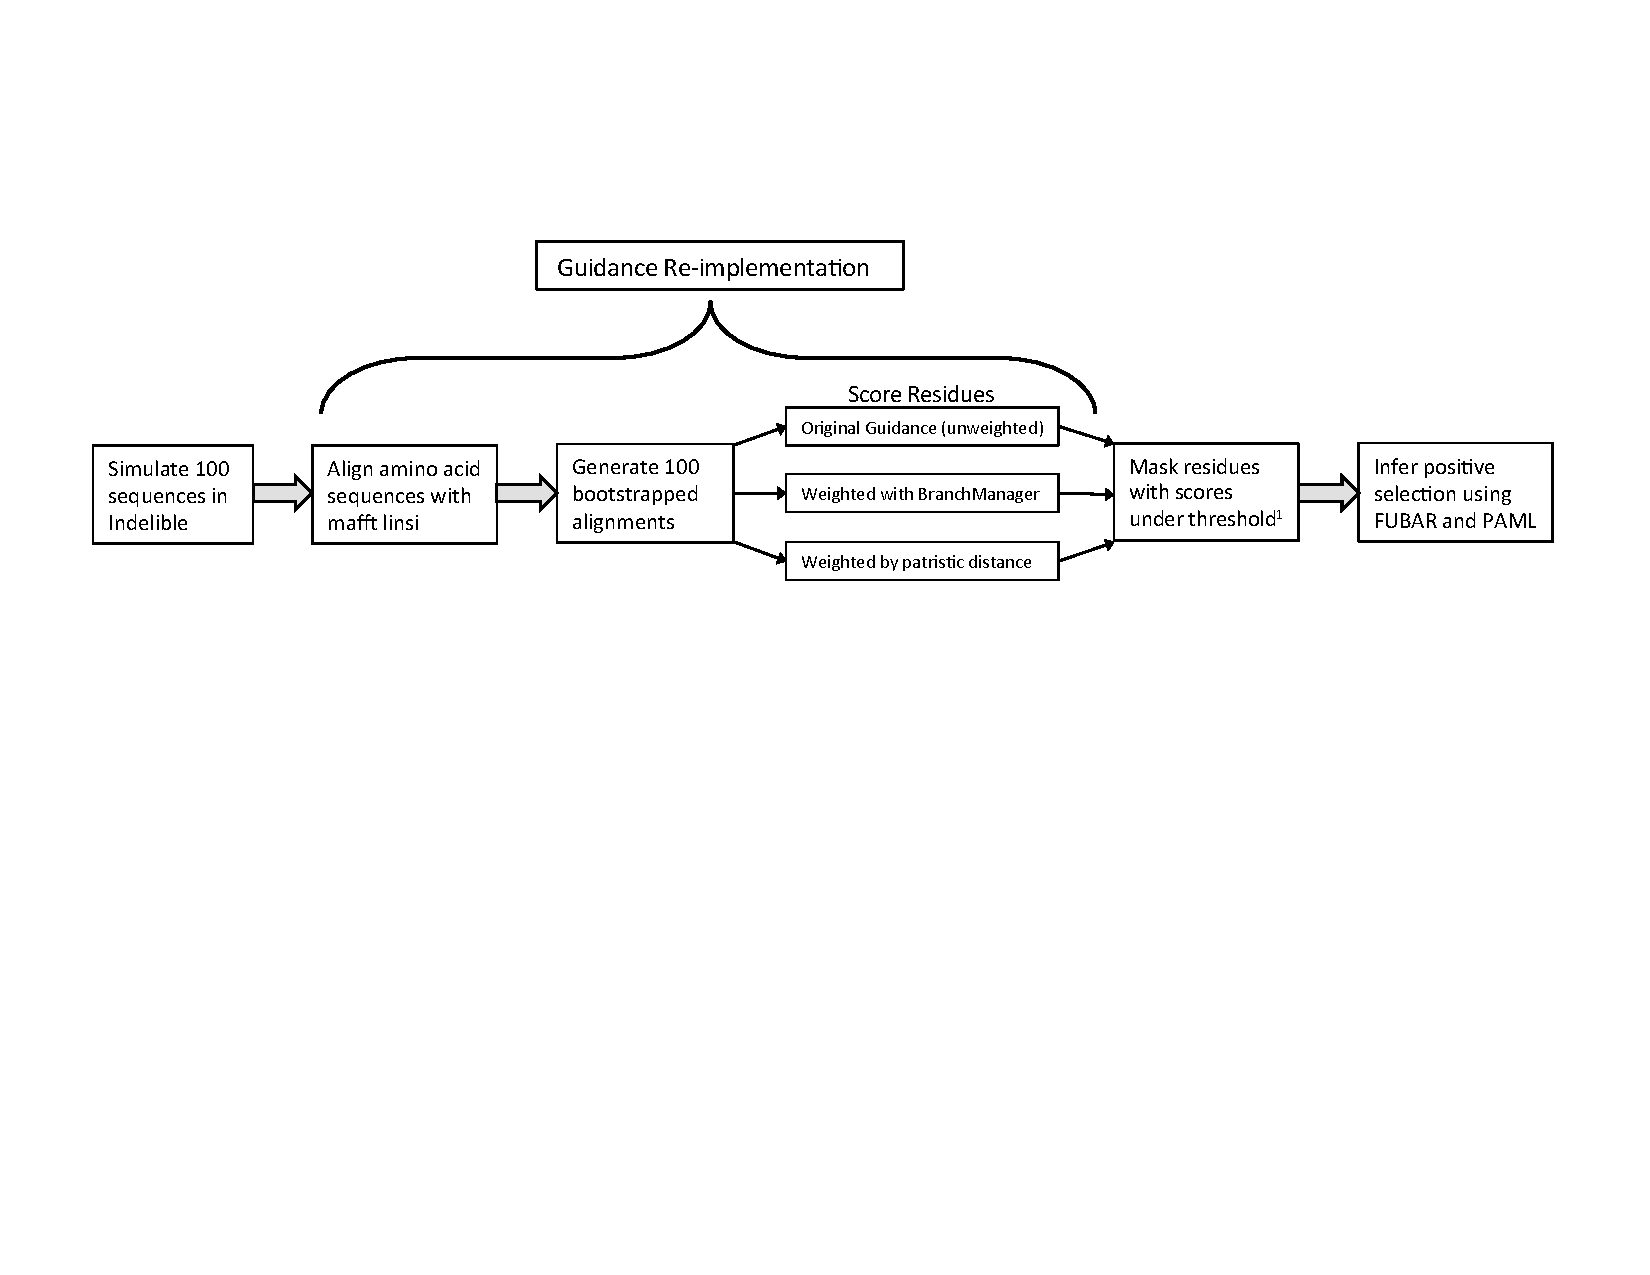
\includegraphics[width=7.5in]{Figures/pipeline.pdf}}
\caption{INSERT CAPTION HERE.}
\label{pipeline} 
\end{figure*}

\begin{figure*}[H]
\centerline{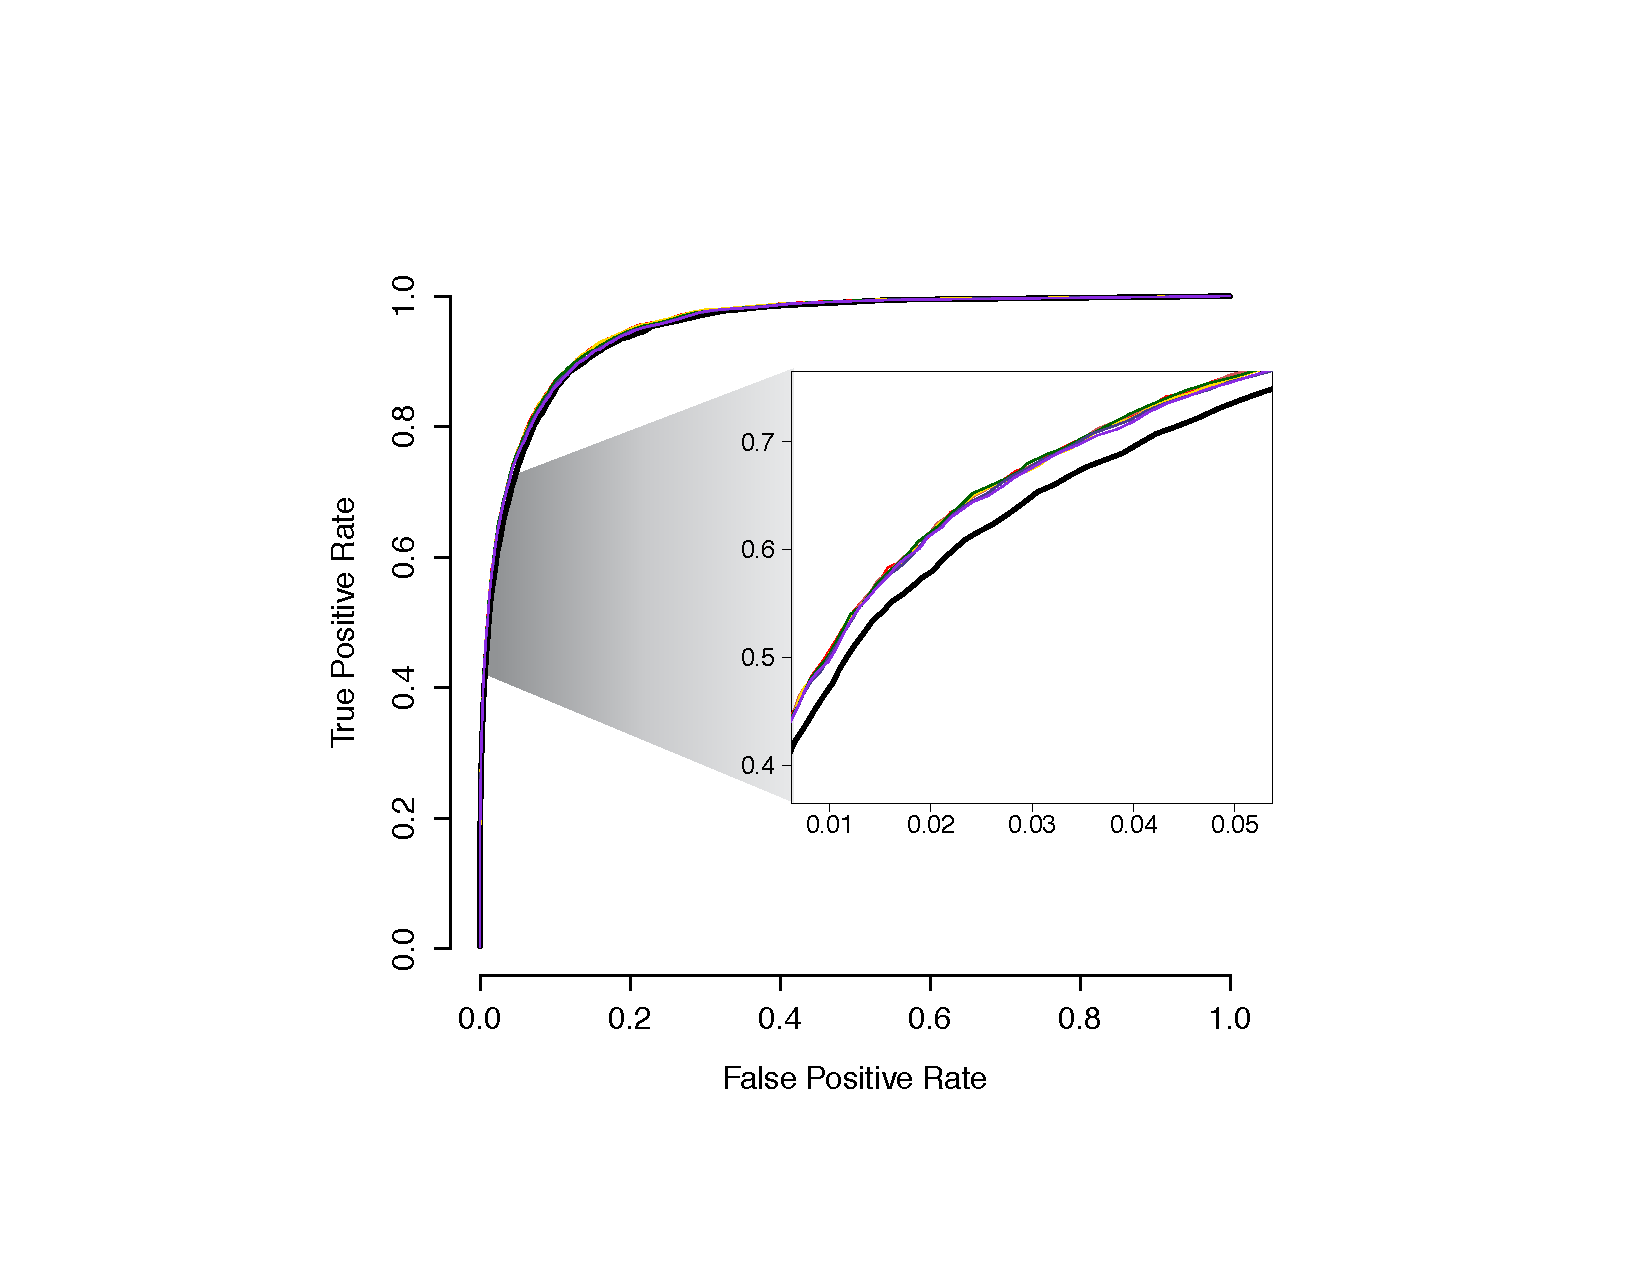
\includegraphics[width=4in]{Figures/fubar_inset_ROC.pdf}}
\caption{INSERT CAPTION HERE. No algorithm clearly stands out. Roughly 3\% above the reference alignment curve. So minimal!}
\label{rocfubar60} 
\end{figure*}



\bibliographystyle{MBE}
\bibliography{citations}	

\end{document}